\documentclass[aspectratio=169]{../latex_main/tntbeamer}  % you can pass all options of the beamer class, e.g., 'handout' or 'aspectratio=43'
\usepackage{dsfont}
\usepackage{bm}
\usepackage[english]{babel}
\usepackage[T1]{fontenc}
%\usepackage[utf8]{inputenc}
\usepackage{graphicx}
\graphicspath{ {./figures/} }
\usepackage{algorithm}
\usepackage[ruled,vlined,algo2e,linesnumbered]{algorithm2e}
\usepackage{hyperref}
\usepackage{booktabs}
\usepackage{mathtools}

\usepackage{amsmath,amssymb}

\DeclareMathOperator*{\argmax}{arg\,max}
\DeclareMathOperator*{\argmin}{arg\,min}

\usepackage{amsbsy}
\newcommand{\vect}[1]{\bm{#1}}
%\newcommand{\vect}[1]{\boldsymbol{#1}}

\usepackage{pgfplots}
\pgfplotsset{compat=1.16}
\usepackage{tikz}
\usetikzlibrary{trees} 
\usetikzlibrary{shapes.geometric}
\usetikzlibrary{positioning,shapes,shadows,arrows,calc,mindmap}
\usetikzlibrary{positioning,fadings,through}
\usetikzlibrary{decorations.pathreplacing}
\usetikzlibrary{intersections}
\pgfdeclarelayer{background}
\pgfdeclarelayer{foreground}
\pgfsetlayers{background,main,foreground}
\tikzstyle{activity}=[rectangle, draw=black, rounded corners, text centered, text width=8em]
\tikzstyle{data}=[rectangle, draw=black, text centered, text width=8em]
\tikzstyle{myarrow}=[->, thick, draw=black]

% Define the layers to draw the diagram
\pgfdeclarelayer{background}
\pgfdeclarelayer{foreground}
\pgfsetlayers{background,main,foreground}

% Requires XeLaTeX or LuaLaTeX
%\usepackage{unicode-math}

\usepackage{fontspec}
%\setsansfont{Arial}
\setsansfont{RotisSansSerifStd}[ 
Path=../latex_main/fonts/,
Extension = .otf,
UprightFont = *-Regular,  % or *-Light
BoldFont = *-ExtraBold,  % or *-Bold
ItalicFont = *-Italic
]
\setmonofont{Cascadia Mono}[
Scale=0.8
]

% scale factor adapted; mathrm font added (Benjamin Spitschan @TNT, 2021-06-01)
%\setmathfont[Scale=1.05]{Libertinus Math}
%\setmathrm[Scale=1.05]{Libertinus Math}

% other available math fonts are (not exhaustive)
% Latin Modern Math
% XITS Math
% Libertinus Math
% Asana Math
% Fira Math
% TeX Gyre Pagella Math
% TeX Gyre Bonum Math
% TeX Gyre Schola Math
% TeX Gyre Termes Math

% Literature References
\newcommand{\lit}[2]{\href{#2}{\footnotesize\color{black!60}[#1]}}

%%% Beamer Customization
%----------------------------------------------------------------------
% (Don't) Show sections in frame header. Options: 'sections', 'sections light', empty
\setbeamertemplate{headline}{empty}

% Add header logo for normal frames
\setheaderimage{
	% 
\includegraphics[height=\logoheight]{figures/TNT_darkv4.pdf}
	
\includegraphics[height=\logoheight]{../latex_main/figures/luh_logo_rgb_0_80_155.pdf}
	% 
\includegraphics[height=\logoheight]{figures/logo_tntluh.pdf}
}

% Header logo for title page
\settitleheaderimage{
	% 
\includegraphics[height=\logoheight]{figures/TNT_darkv4.pdf}
	
\includegraphics[height=\logoheight]{../latex_main/figures/luh_logo_rgb_0_80_155.pdf}
	% 
\includegraphics[height=\logoheight]{figures/logo_tntluh.pdf}
}

% Title page: tntdefault 
\setbeamertemplate{title page}[tntdefault]  % or luhstyle
% Add optional title image here
%\addtitlepageimagedefault{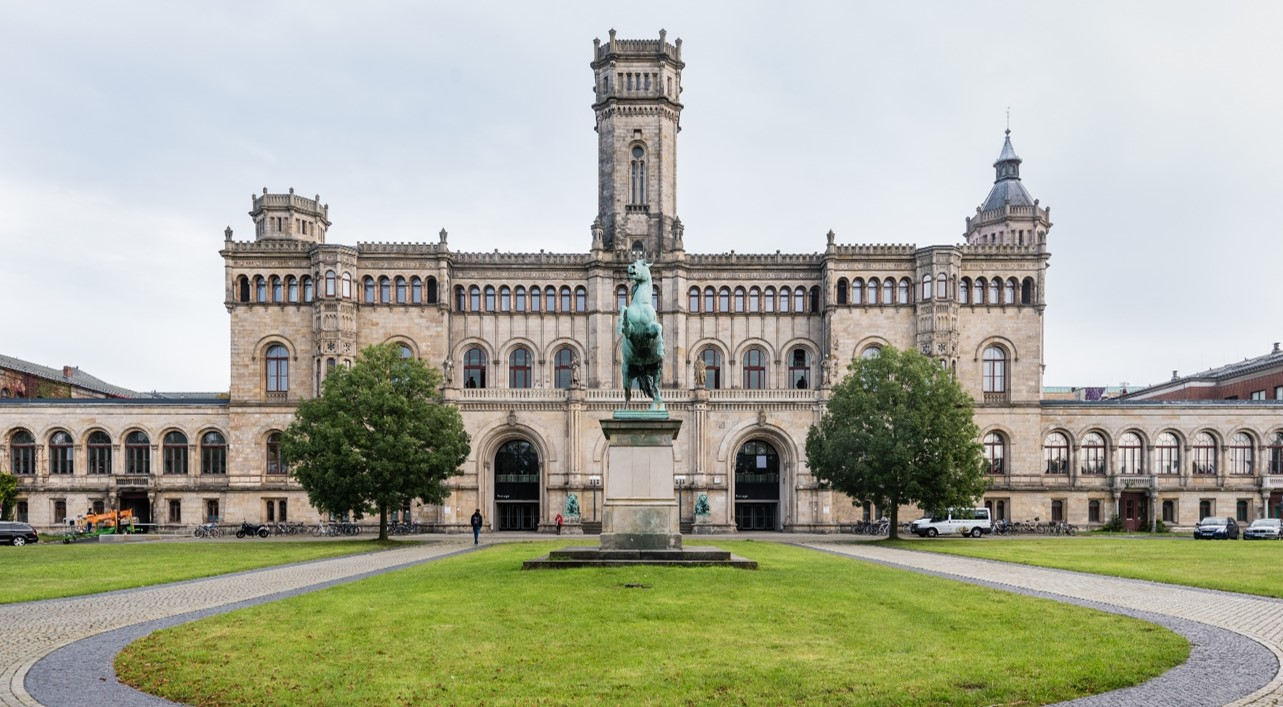
\includegraphics[width=0.65\textwidth]{figures/luh_default_presentation_title_image.jpg}}

% Title page: luhstyle
% \setbeamertemplate{title page}[luhstyle]
% % Add optional title image here
% \addtitlepageimage{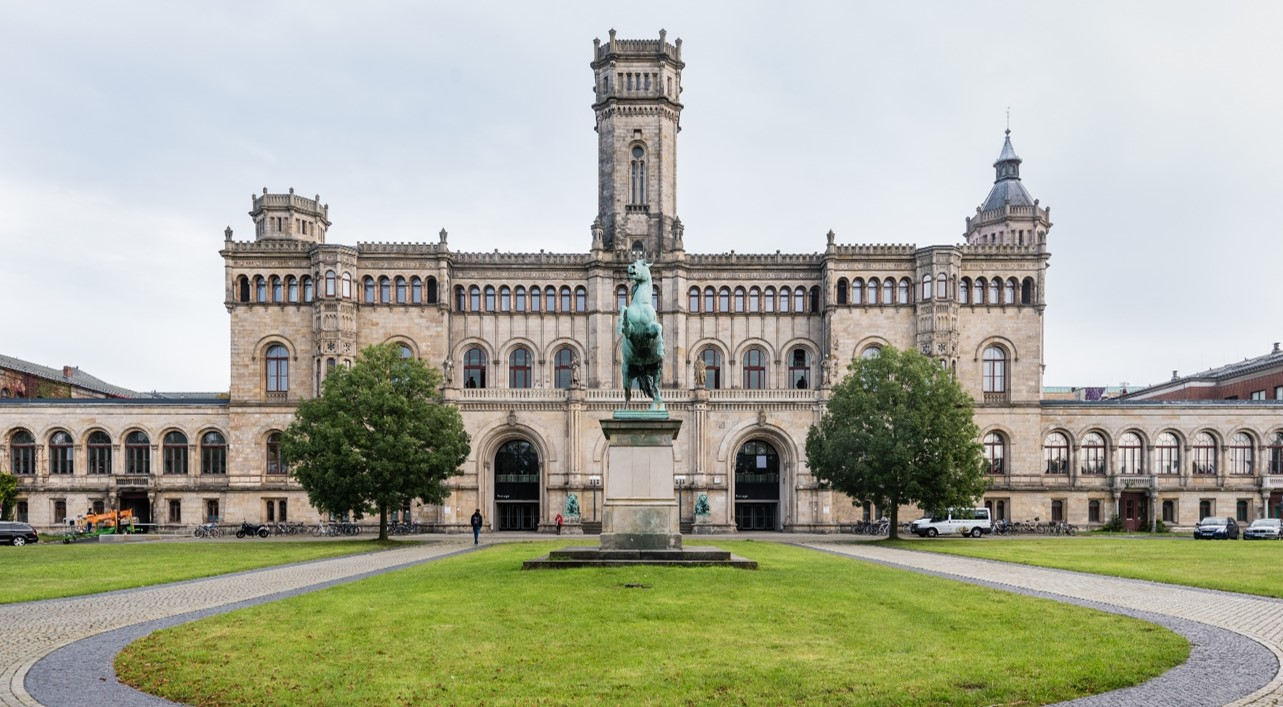
\includegraphics[width=0.75\textwidth]{figures/luh_default_presentation_title_image.jpg}}

\author[Abedjan \& Lindauer]{Ziawasch Abedjan \& Marius Lindauer\\[1em]
	
\includegraphics[height=\logoheight]{../latex_main/figures/luh_logo_rgb_0_80_155.pdf}\qquad
	
\includegraphics[height=\logoheight]{../latex_main/figures/DBIS_Kurzlogo.png}\qquad

\includegraphics[height=\logoheight]{../latex_main/figures/TNT_darkv4}\qquad

\includegraphics[height=\logoheight]{../latex_main/figures/L3S.jpg}	}
\date{Summer Term 2022; \hspace{0.5em} {
\includegraphics[height=1.5em]{../latex_main/figures/Cc-by-nc-sa_icon.svg.png}}; based on \href{https://ds100.org/fa21/}{[DS100]}
}


%%% Custom Packages
%----------------------------------------------------------------------
% Create dummy content
\usepackage{blindtext}

% Adds a frame with the current page layout. Just call \layout inside of a frame.
\usepackage{layout}


%%% Macros
%\renewcommand{\vec}[1]{\mathbf{#1}}
% \usepackage{bm}
%\let\vecb\bm

\title[Introduction]{DS: Decision Trees}
\subtitle{Decision Trees in scikit-learn}

\graphicspath{ {./figure/} }
%\institute{}


\begin{document}
	
	\maketitle
	\begin{frame}{Decision Tree Models With scikit-learn }
	    The code to build a decision tree model in scikit-learn is very similar to what we saw for building linear and logistic regression models:
	    \begin{figure}
	        \centering
	        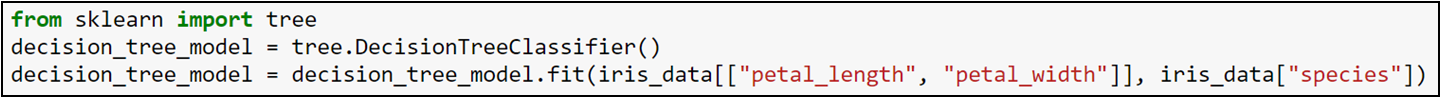
\includegraphics[scale=.6]{Bild17}
	    \end{figure}
	    See lec20-decision-trees.ipynb if you want to try it out
	\end{frame}
	
	
	
	\begin{frame}{Decision Tree Models With scikit-learn }
	    The code to build a decision tree model in scikit-learn is very similar to what we saw for building linear and logistic regression models:
	    \begin{figure}
	        \centering
	        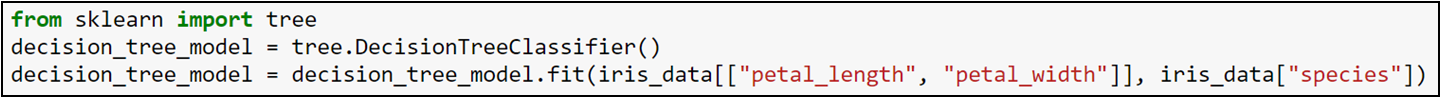
\includegraphics[scale=.6]{Bild17}
	    \end{figure}
	    See lec20-decision-trees.ipynb if you want to try it out
        \begin{figure}
            \centering
            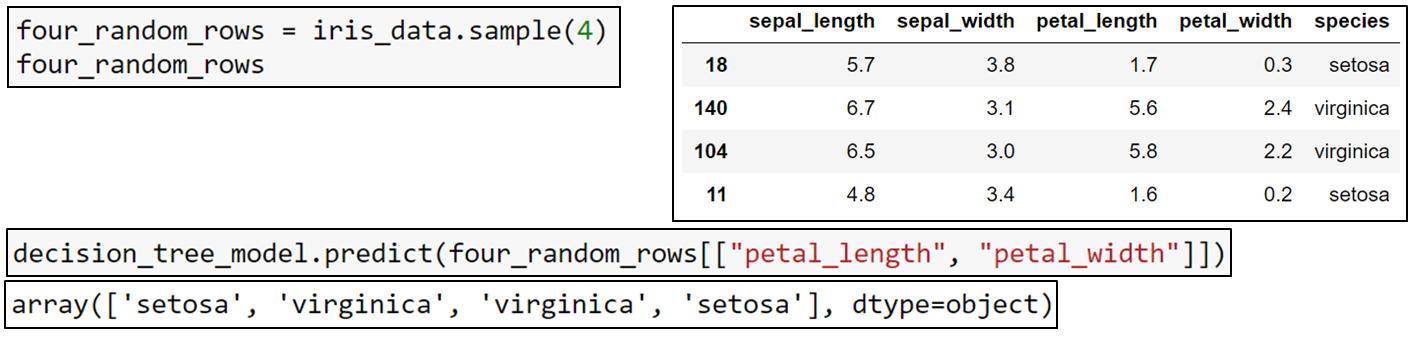
\includegraphics[scale=.4]{Bild18}
        \end{figure}
	\end{frame}
	
	
	\begin{frame}{Visualizing Decision Tree Models }
	    \begin{figure}
	        \centering
	        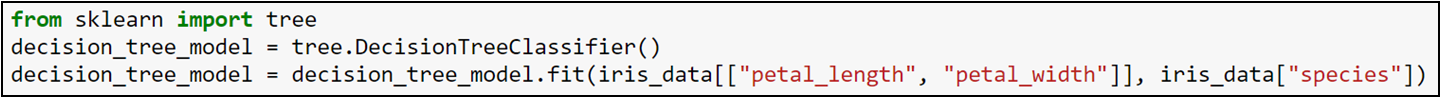
\includegraphics[scale=.6]{Bild17}
	    \end{figure}
	    Suppose we want to visualize the decision tree, similar to what we saw earlier:
        \begin{figure}
            \centering
            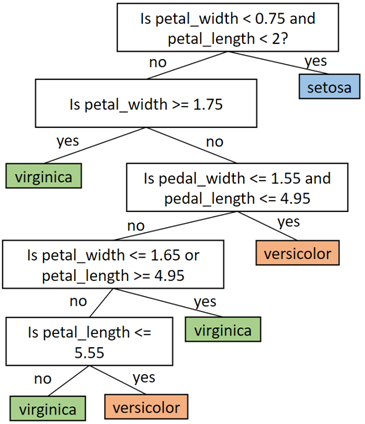
\includegraphics[scale=.65]{Bild19}
        \end{figure}
	\end{frame}
	
	
	\begin{frame}{Visualizing Decision Tree Models }
	    \begin{figure}
	        \centering
	        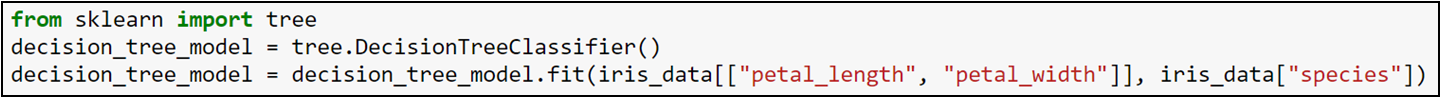
\includegraphics[scale=.6]{Bild17}
	    \end{figure}
	    \begin{columns}
	        \begin{column}{.5\textwidth}
	                \begin{figure}
	                    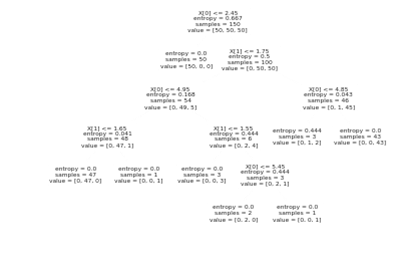
\includegraphics[scale=.55]{Bild22}
	                \end{figure}
	        \end{column}
	        
	        
	        \begin{column}{.5\textwidth}
	                There is a built in DecisionTree visualizer
	                \begin{itemize}
	                    \item Unfortunately, it isn’t very good
	                \end{itemize}
	                \begin{figure}
	                    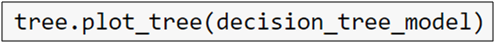
\includegraphics[scale=.65]{Bild21}
	                \end{figure}
	        \end{column}
	    \end{columns}
	\end{frame}
	
	
	\begin{frame}{Visualizing Decision Tree Models }
	    \begin{columns}
	        \begin{column}{.4\textwidth}
	        Can use GraphViz to get a much nicer picture.
	                \begin{figure}
	                    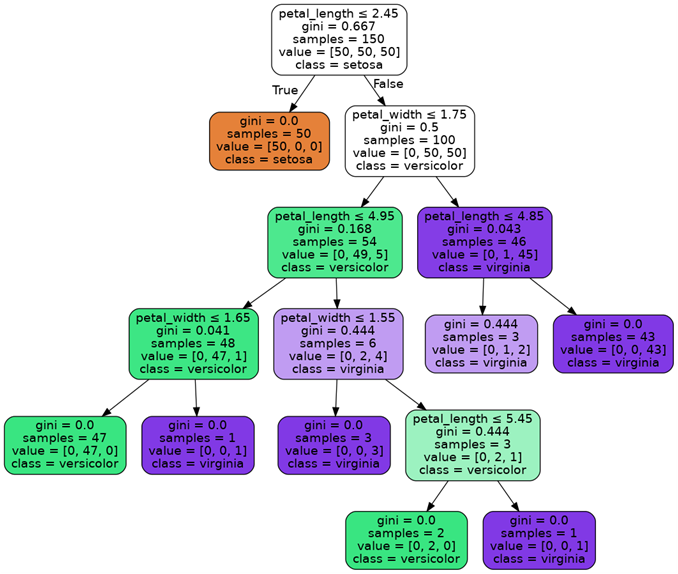
\includegraphics[scale=.5]{Bild23}
	                \end{figure}
	        \end{column}
	        
	        
	        \begin{column}{.6\textwidth}
	                \begin{figure}
	                    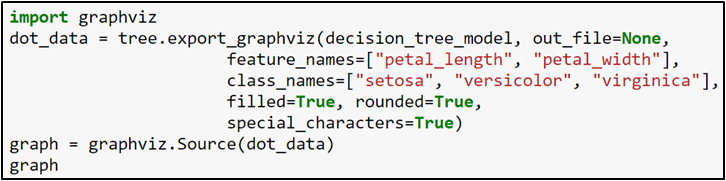
\includegraphics[scale=.55]{Bild24}
	                \end{figure}
	                In each box, we see:
	                \begin{itemize}
	                    \item The rule
	                    \item The gini impurity (chance that a sample would be misclassified if randomly assigned at this point)
	                    \item The number of samples still unclassified
	                    \item The number of samples in each class still unclassified
	                    \item The most likely class
	                \end{itemize}
	        \end{column}
	    \end{columns}
	\end{frame}
	
	
	\begin{frame}{Visualizing Decision Tree Models }
	    \begin{columns}
	        \begin{column}{.4\textwidth}
	        Can use GraphViz to get a much nicer picture.
	                \begin{figure}
	                    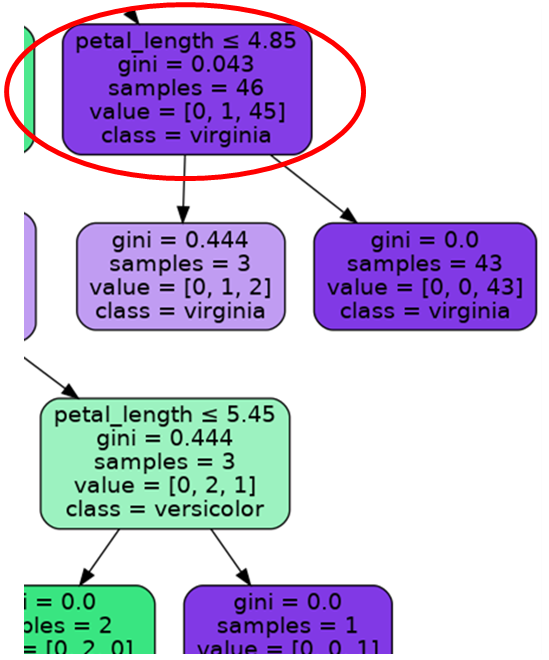
\includegraphics[scale=.3]{Bild25}
	                \end{figure}
	        \end{column}
	        
	        
	        \begin{column}{.6\textwidth}
	                \begin{figure}
	                    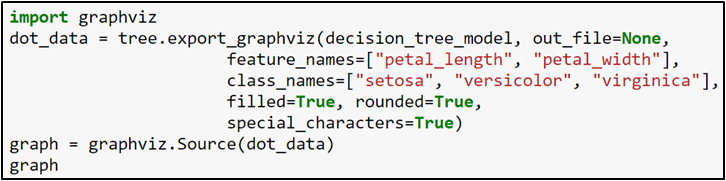
\includegraphics[scale=.55]{Bild24}
	                \end{figure}
	                In each box, we see:
	                \begin{itemize}
	                    \item The rule
	                    \item The gini impurity (chance that a sample would be misclassified if randomly assigned at this point)
	                    \item The number of samples still unclassified
	                    \item The number of samples in each class still unclassified
	                    \item The most likely class
	                \end{itemize}
	        \end{column}
	    \end{columns}
	\end{frame}
	
	
	\begin{frame}{Visualizing Decision Tree Models}
	    Plotting the decision boundaries for our logistic regression \& decision tree models, yields these results:
	    \begin{itemize}
	        \item Decision tree has nonlinear boundary, and appears to get 100\% accuracy
	        \begin{itemize}
	            \item Let’s calculate the exact accuracy rather than just relying on our eyes
	        \end{itemize}
	    \end{itemize}
	    \begin{figure}
	        \centering
	        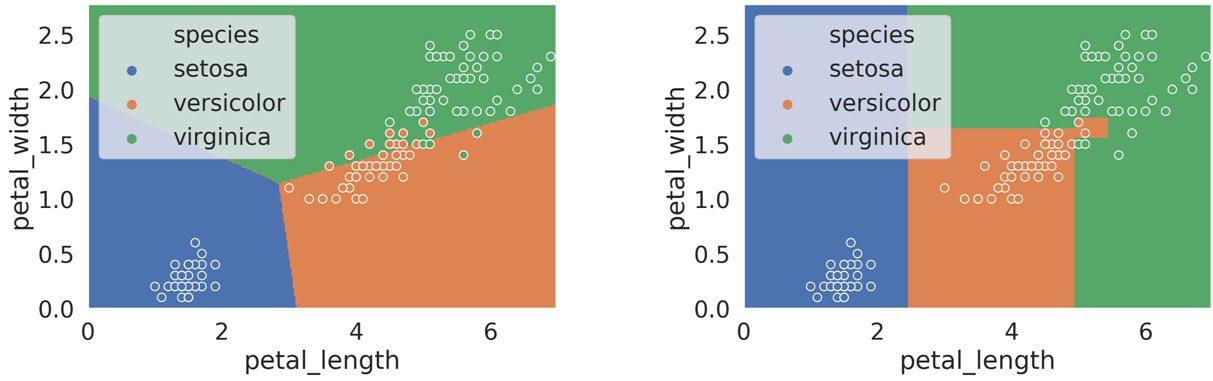
\includegraphics[scale=.45]{Bild26}
	    \end{figure}
	\end{frame}
	
	
	\begin{frame}{Measuring the Performance of Our Model}
	    Running the code below, we see that we only get 99.3% accuracy
        \begin{figure}
            \centering
            
\includegraphics[scale=.65]{Bild27}
        \end{figure}
        To understand why, let’s look back at our decision tree model
	\end{frame}
	
	
	\begin{frame}{Understanding Our Decision Tree}
	    \begin{columns}
	        \begin{column}{.5\textwidth}
	                \begin{figure}
	                    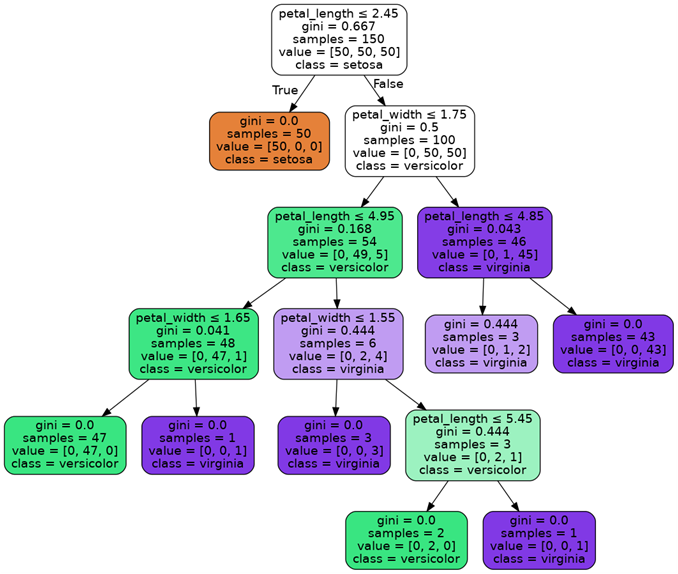
\includegraphics[scale=.55]{Bild23}
	                \end{figure}
	        \end{column}
	        
	        
	         \begin{column}{.5\textwidth}
	                \\ \bigskip \bigskip
	                There is one terminal decision point where there is more than one possible right answer\\
	                \bigskip
	                Can you find it?
	        \end{column}
	    \end{columns}
	\end{frame}
	
	
	
	
	\begin{frame}{Understanding Our Decision Tree}
	    \begin{columns}
	        \begin{column}{.5\textwidth}
	                \begin{figure}
	                    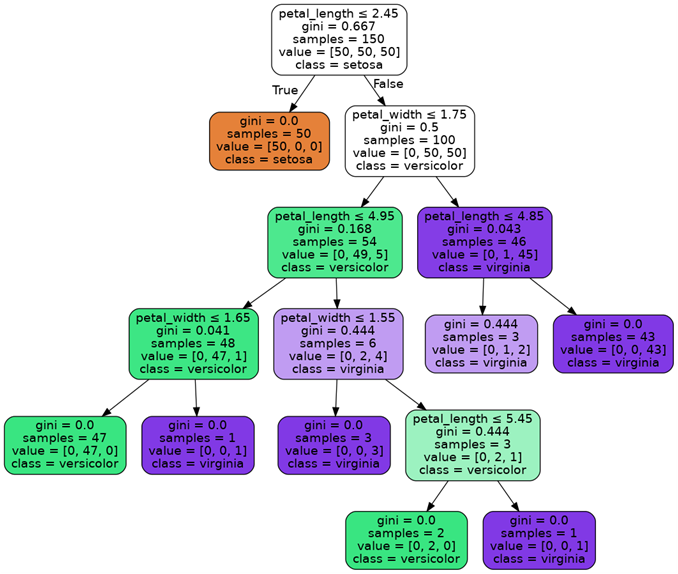
\includegraphics[scale=.55]{Bild23}
	                \end{figure}
	        \end{column}
	        
	        
	         \begin{column}{.5\textwidth}
	                \\ \bigskip \bigskip
	                There is one terminal decision point where there is more than one possible right answer\\
	                \bigskip
	                The model was unable to come up with a decision rule to resolve these last 3 samples\\
	                \bigskip
	                Let’s see why using the query method of the dataframe class
	        \end{column}
	    \end{columns}
	\end{frame}
	
	
	\begin{frame}{Understanding Our Decision Tree}
	                \begin{figure}
	                    
\includegraphics[scale=.3]{Bild28}
	                \end{figure}
	    \begin{columns}
	        \begin{column}{.4\textwidth}
	                \begin{figure}
	                    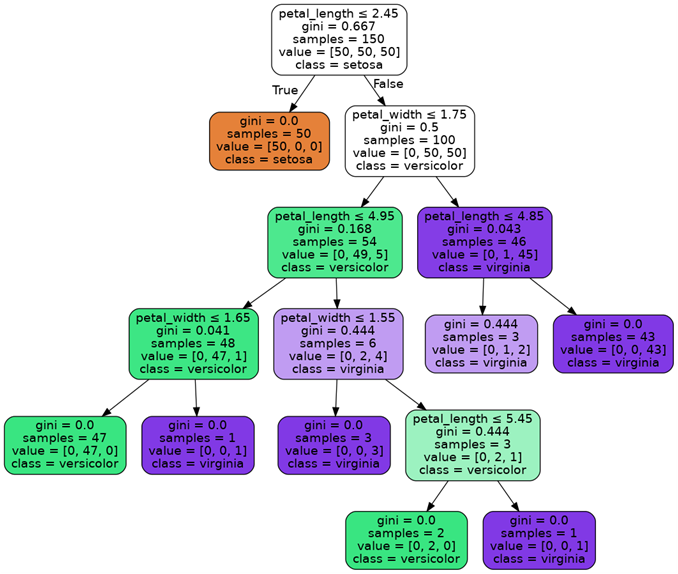
\includegraphics[scale=.35]{Bild23}
	                \end{figure}
	        \end{column}
	        
	        
	         \begin{column}{.4\textwidth}
	                There is one terminal decision point where there is more than one possible right answer
	                \begin{itemize}
	                    \item In the original data set, there was a versicolor iris with the same petal measurements as two virginicas
	                \end{itemize}
	        \end{column}
	    \end{columns}
	\end{frame}
	
	
	
	\begin{frame}{Overfitting and Decision Trees}
	    Bottom line: scikit-learn makes it easy to generate decision trees
	    \begin{figure}
	        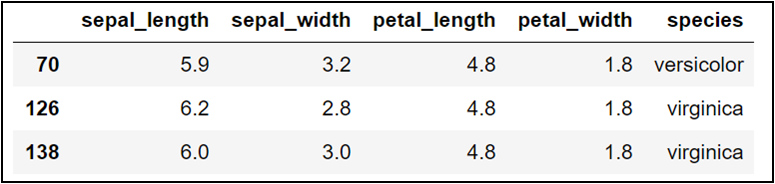
\includegraphics[scale=.5]{Bild29}
	    \end{figure}
	    These decision trees will always have perfect accuracy on the training data, EXCEPT when there are samples from different categories with the exact same features
	    \begin{itemize}
	        \item That is, if the versicolor above had a petal\_length of 4.800001, we’d have 100\% training accuracy
	    \end{itemize}
	    
	    \bigskip
	    This tendency for perfect accuracy should give us concern about overfitting
	\end{frame}
\end{document}